 
\begin{figure}[h]
\centering
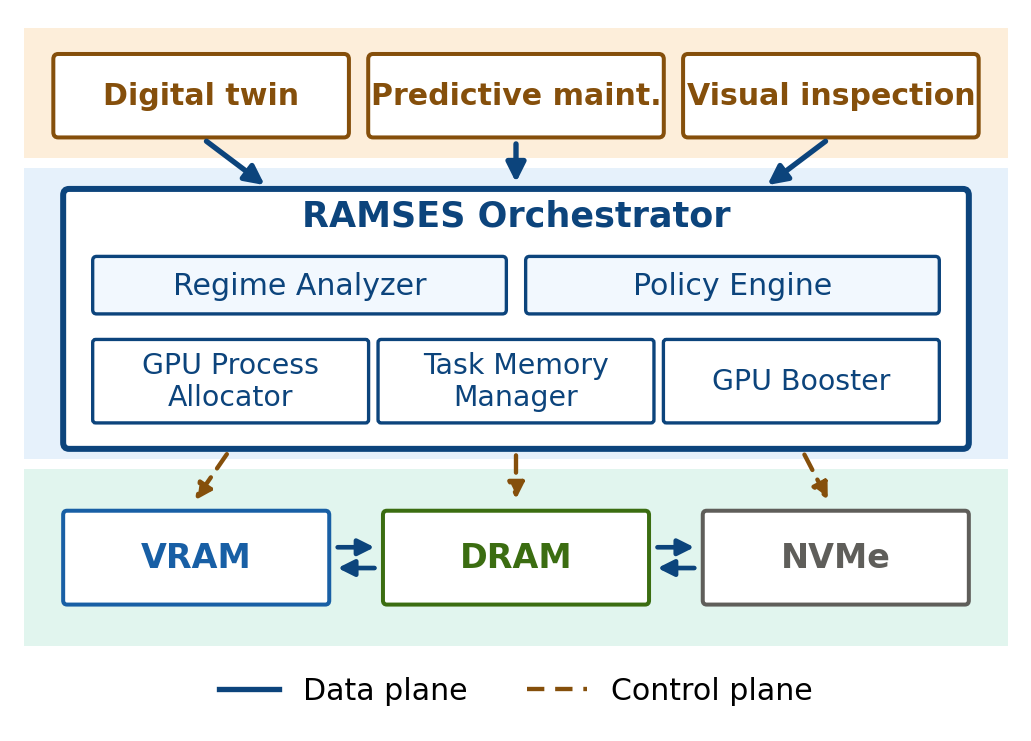
\includegraphics[width=0.72\linewidth]{figures/rameses_design.png}
\caption{Industrial hierarchical memory architecture of RAMSES
for laboratory workloads motivated by industrial analytics.
The data plane (solid arrows) coordinates GPU VRAM, host DRAM,
and NVMe for three industrial workloads:
(1) digital twin state synchronization aligned with PLC scan cycles,
(2) predictive maintenance triggered by anomaly bursts from IIoT sensors,
and (3) real-time visual inspection under bounded inference deadlines.
The control plane (dashed arrows) includes a Regime Analyzer
estimating $(\alpha,\beta)$ and a Policy Engine enforcing tier-aware
placement, prefetch, and swap decisions.
Three modules handle the actual orchestration:
the \emph{GPU Process Allocator} pre-reserves CUDA context to remove
context-conflict stalls,
the \emph{Task Memory Manager} performs NUMA-aware allocation with
predictive DRAM offloading,
and the \emph{GPU Booster} drives block-aligned asynchronous VRAM--NVMe
swap.
The diagram supplies workload motivation only; it does not depict a deployed control loop, TSN integration, or a validated hard deadline.}
\label{fig:rameses_architecture}
\end{figure}

\section{RAMSES: Architecture and Key Components}\label{sec:mball}
\footnotetext[1]{The anonymized review artifact bundles the \texttt{LD\_PRELOAD} orchestrator layer, the synthetic-trace generator, baseline invocation scripts, the request-level measurement schema, and the analysis programs used to produce the reported results.}

LLM inference couples GPUs, VRAM, DRAM, NVMe, and Central Processing Units (CPUs), yet serving stacks rarely treat resource contention as first-class, producing recurring Compute Unified Device Architecture (CUDA) out-of-memory (OOM) errors, context-switch stalls, and memory-mapping overhead. Prior GPU--CPU offloading~\cite{xu2025ellm}, speculative offloading~\cite{zhuge2025specoffload}, and cache-centric management~\cite{jiang2024neo} mostly stop at single-tier (VRAM--CPU) transfers or narrow scenarios such as key-value (KV) cache management.

\textbf{RAMSES} applies the OS notion of memory ballooning to LLM serving, managing the whole VRAM--DRAM--NVMe hierarchy in one control loop---GPU context conflicts, NUMA-induced latency, and inefficient swapping addressed together rather than patched independently---while staying lightweight enough to avoid a full distributed framework. Three modules form the core---the \textbf{GPU Process Allocator}, the \textbf{Task Memory Manager}, and the \textbf{GPU Booster with swap support}---illustrated in Fig.~\ref{fig:rameses_architecture}.

\subsection{GPU Process Allocator}
In multi-model serving, two bottlenecks dominate: \textbf{GPU context loading conflicts} and \textbf{VRAM interference}. CUDA drivers do context initialization and memory mapping with \textit{lazy binding}, which is fine for a single workload but becomes painful under concurrent execution---startup delays grow, and they show up directly in user-facing latency. NEO \cite{jiang2024neo} addresses cache management but leaves the GPU-level context conflict question open.
The \textbf{GPU Process Allocator} resolves these conflicts ahead of time rather than at runtime, through three policies. (i)~\emph{Pre-defined slot reservation} pre-assigns each model a context ID, memory pool, and kernel queue, removing CUDA initialization from the critical path. (ii)~\emph{Context separation with fixed memory pools} places models in disjoint regions, lowering fragmentation and cross-model cache interference. (iii)~\emph{Priority-based scheduling} co-schedules I/O-bound and compute-bound models so neither stalls the other and idle GPU cycles shrink. The net effect is a lightweight extension of process pinning that improves QoS stability and latency predictability when several models share one GPU~\cite{stojkovic2025dynamollm}.



\subsection{Task Memory Manager}
Memory usage during LLM inference shifts back and forth between DRAM and VRAM as input and generation lengths change. eLLM \cite{xu2025ellm} responded to this by extending the CPU buffer; PIE \cite{xu2024pie} took a speculative-swap approach. Neither, though, paid attention to NUMA-induced latency or to optimization within DRAM itself.

Our \textbf{Task Memory Manager} pairs task-level memory control with four NUMA-aware mechanisms. \emph{NUMA-aware mapping} pins process and thread data to local nodes via \texttt{mbind()} and \texttt{numa\_alloc\_onnode()} to minimize remote traffic; a \emph{jemalloc-based heap} separates small objects from large tensors to bound fragmentation~\cite{hunter2021hugepage,yang2023numalloc}; \emph{task-level redistribution} offloads non-critical tensors to DRAM before VRAM saturates; and a \emph{lightweight pressure predictor} reads live utilization and I/O-queue depth to trigger mitigation early~\cite{korthikanti2023reducing}. We model memory-access latency as $T_{access}=T_{local}+\gamma\,T_{remote}$, with $\gamma$ the remote-NUMA penalty. Poor allocation here cascades into excessive page reclaim, \texttt{mmap} failures, and buffer eviction; reactive offloading or compression leaves DRAM behavior and NUMA locality unaddressed. Together these keep DRAM--VRAM use efficient under contention, with less fragmentation and fewer page-reclaim events.



\begin{table}[t]
\centering
\renewcommand{\arraystretch}{1.05}
\caption{Baselines compared against RAMSES: key technique and the RAMSES module that targets each bottleneck. Citations refer to the baseline systems.}
\label{tab:baseline_comparison}
\footnotesize
\setlength{\tabcolsep}{3pt}
\begin{tabular}{@{}p{1.95cm}p{2.5cm}p{3.1cm}@{}}
\toprule
\textbf{Method} & \textbf{Key technique} & \textbf{Targeted by RAMSES} \\
\midrule
PyTorch (default) & none & overall gain \\
FlexGen~\cite{sheng2023flexgen} & CPU offloading & GPU Booster (swap) \\
SwapAdvisor~\cite{swapAdvisor2020} & GPU--CPU swap & Task Memory Manager \\
NEO~\cite{jiang2024neo} & KV offload + sched. & full-tier use \\
SpecOffload~\cite{zhuge2025specoffload} & cross-tier swap & NVMe--VRAM path \\
vLLM~\cite{kwon2023pagedattention} & KV cache + stream & end-to-end latency \\
\bottomrule
\end{tabular}
\end{table}

\subsection{GPU Booster with Swap Support}
FlexGen~\cite{sheng2023flexgen} and SwapAdvisor~\cite{swapAdvisor2020} support GPU--CPU swapping but are not tuned to GPU memory hierarchies. The \textbf{GPU Booster} targets VRAM capacity by selecting inactive tensors for block-aligned asynchronous transfer, implemented as an \texttt{LD\_PRELOAD} layer over the CUDA runtime and caching allocator: allocation, free, and host--device copy calls are intercepted so placement is managed without modifying the model or framework (intercepted entry points, buffer registration, and driver/filesystem versions are in the artifact).

Unlike OS-level swapping, which is unaware of GPU memory semantics, the GPU Booster ranks eviction candidates by execution-graph reuse distance, overlaps transfer with compute on dedicated asynchronous CUDA streams, and uses 4~MB block alignment matched to the NVMe erase-block granularity (examined in the sensitivity study of Section~\ref{sec:results}). Where GPUDirect Storage is available, tensors move over a direct VRAM--NVMe DMA path; otherwise the layer falls back to a pinned-host-buffer staged path with the same overlap. Partial reload fetches only the portion of a swapped tensor the next kernel needs, and output equivalence against the baseline is checked bitwise for FP32 and within tolerance for FP16.

The goal is to serve models whose state exceeds VRAM capacity while keeping exposed transfer latency low. All three module procedures are summarized in Algorithm~\ref{alg:ramses}.

\begin{algorithm}[t]
\caption{RAMSES module procedures}
\label{alg:ramses}
\scriptsize
\begin{algorithmic}[1]
\Procedure{GPUProcessAllocator}{models $\mathcal{M}$, pool $\mathcal{R}$}
  \State Initialize free context IDs, memory pools, kernel queues
  \For{each $m\in\mathcal{M}$}
    \State Reserve context/pool/queue; set priority (I/O- vs compute-bound)
  \EndFor
  \While{tasks remain}
    \State Dequeue by priority; launch on reserved context; free on completion
  \EndWhile
\EndProcedure
\Procedure{TaskMemoryManager}{graph $G$, threshold $\tau$}
  \State Bind threads to local NUMA nodes; split jemalloc heaps (small/large)
  \For{each request $r$}
    \If{VRAM usage $>\tau$} \State offload low-reuse tensors of $G$ to DRAM/NVMe \EndIf
    \State Predict pressure from utilization/I-O depth; pre-allocate next request
  \EndFor
\EndProcedure
\Procedure{GPUBooster}{graph $G$}
  \For{each inactive tensor $t\in G$}
    \State 4\,MB-align; async DMA $t\!\to\!$NVMe; mark swapped-out
  \EndFor
  \While{serving}
    \State On reaching a swapped $t$: partial async reload, then resume
  \EndWhile
\EndProcedure
\end{algorithmic}
\end{algorithm}


%----------------------------------------------------------------


\subsection{Overlap-Aware Operating Model}\label{sec:theory}

{\revcolor
We use the following model as an engineering classification tool, not as a
real-time guarantee.  Let $D(t)$ be the bytes resident or demanded by a step,
$C_f=C_{\mathrm{VRAM}}+C_{\mathrm{DRAM}}$ the usable fast-tier capacity,
$V_{\uparrow}(t)$ and $V_{\downarrow}(t)$ the measured read and write transfer
volumes, $h(t)$ the prefetch-hit fraction, and $q(t)$ the measured storage
queueing delay.  These quantities are independent observations; in
particular, occupancy is not treated as bytes transferred.  The capacity
pressure is
\begin{equation}\label{eq:alpha_def}
 \alpha(t)=D(t)/C_f,
\end{equation}
and the transfer pressure is
\begin{equation}\label{eq:beta_def}
 \beta(t)=\frac{L_0+q(t)+V_{\uparrow}(t)/B_{\uparrow}
 +V_{\downarrow}(t)/B_{\downarrow}}
 {T_{\mathrm{comp}}(t)+T_{\mathrm{mem}}(t)+T_{\mathrm{sync}}(t)}.
\end{equation}
Here $L_0$ is fixed request/setup latency and $B_{\uparrow}$ and
$B_{\downarrow}$ are effective, direction-specific bandwidths measured with
the same block size and queue depth as the experiment.  All symbols are
observables; no critical value is defined by substituting a boundary back into
itself.

Asynchronous transfer overlaps computation.  Accordingly, predicted service
time is
\begin{IEEEeqnarray}{rCl}\label{eq:latency_total}
\widehat T_{\mathrm{total}} &=& T_{\mathrm{{sync}}}+T_{\mathrm{mem}}
 +\max\{T_{\mathrm{comp}},(1-h)T_{\mathrm{xfer}}\},\\
T_{\mathrm{xfer}}&=&L_0+q+V_{\uparrow}/B_{\uparrow}+V_{\downarrow}/B_{\downarrow}.
\end{IEEEeqnarray}
The max operator prevents double counting overlapped DMA and compute.  Block
rounding is included in the measured volumes.  We call observations with
$\alpha>1$ capacity-limited and observations with $\beta\geq1$ transfer-
limited; the remaining points are coordination-dominated.  These are
operational labels, not theorems.  They neither imply zero swapping nor a
worst-case bound.  Fig.~\ref{fig:phase_measured} summarizes the resulting
classification.  Section~\ref{sec:results} reports the operating regime the
evaluated systems occupy; per-request measured $(\alpha,\beta)$ values and the
residual of Eq.~\eqref{eq:latency_total} against end-to-end latency are logged
by the instrumentation of Section~\ref{sec:latency_protocol} and released with
the artifact.

}

\subsection{Online Policy and Complexity}\label{sec:controller}
{\revcolor
Every 200~ms the analyzer reads allocated bytes, transfer counters, queue
depth, effective bandwidth, and exponentially weighted compute, memory, and
synchronization times.  It computes Eqs.~\eqref{eq:alpha_def}--\eqref{eq:beta_def}
in constant time.  To avoid oscillation, a state change requires three
consecutive samples beyond a 5\% hysteresis band.  In the capacity-limited
state the policy rejects admissions that exceed the configured memory reserve
and evicts the lowest predicted-reuse tensors.  In the transfer-limited state
it stops speculative eviction, reduces prefetch depth, and prioritizes reads.
In the coordination-dominated state it enables asynchronous prefetch and
NUMA-local placement.  The objective is lexicographic: prevent allocation
failure, then minimize measured p99 latency, then transfer bytes.

The reuse score is an exponentially weighted count of accesses over the last
32 graph steps; it has no learned parameters or offline training.  Candidate
maintenance costs $O(\log n)$ per tensor access for a heap of $n$ evictable
tensors; sampling, regime classification, and a policy decision are $O(1)$,
and metadata occupies $O(n)$.  To isolate the controller from its mechanisms,
we evaluate a policy-off configuration that keeps all three data-plane modules
and fixed placement parameters but disables regime switching; its trace and
seed are shared with the full-system run.  Disabling the policy forfeits the
coordination-region behavior, so the system drifts toward the transfer-limited
boundary under burst load, consistent with the sustained-load results in
Section~\ref{sec:results}; the paired per-run records are included in the
artifact.  The measured 1.68~ms is mean controller work per serving request
and is not compatible with a 2~ms end-to-end claim; we therefore make no such
claim.

}

\subsection{Scope of Timing and Safety Claims}
{\revcolor
The measured latency distributions are QoS observations for non-safety AI
serving.  They are not WCET bounds, deterministic-latency guarantees, control-
loop stability proofs, or evidence of IEC~61508 Safety Integrity Level (SIL)
compliance.  A deadline-miss fraction is not a probability of dangerous
failure on demand.  Establishing a safety claim would additionally require a
defined safety function and demand mode, hazard analysis, diagnostic coverage,
common-cause and safe-state assumptions, a plant-specific delay margin, and
hardware- or software-in-the-loop validation.  RAMSES must therefore be kept
outside a safety function unless independently qualified by the integrator.

}

\subsection{Ablation Analysis}
\rev{We ablate the three modules over four configurations (Table~\ref{tab:ablation}); every ablation degrades performance, and each module dominates the metric it targets. Removing the \textbf{GPU Process Allocator} has the largest latency impact (35.0\%$\rightarrow$20.5\%, $-$14.5~pp), matching its role of pre-resolving CUDA context conflicts on the critical path; removing the \textbf{Task Memory Manager} has the largest VRAM impact (15.0\%$\rightarrow$5.0\%, $-$10.0~pp), matching its NUMA-aware allocation and predictive offloading; and disabling the \textbf{GPU Booster} degrades both intermediately, matching its VRAM--NVMe swap role~\cite{korthikanti2023reducing}.}

\begin{table}[h]
\centering
\renewcommand{\arraystretch}{1.0}
\caption{Ablation study results: Impact of disabling RAMSES modules}
\label{tab:ablation}
\footnotesize
\begin{tabular}{|l|c|c|c|}
\hline
\textbf{Configuration} &
\makecell{\textbf{Load Time} \\ \textbf{Reduction}} &
\makecell{\textbf{Latency} \\ \textbf{Reduction}} &
\makecell{\textbf{VRAM} \\ \textbf{Reduction}} \\
\hline
Full RAMSES             & 58.7$\pm$1.8\% & 35.0$\pm$1.2\% & 15.0$\pm$0.9\% \\
Without GPU Allocator  & 40.1$\pm$2.1\% & 20.5$\pm$1.6\% & 14.1$\pm$1.0\% \\
Without Memory Manager & 45.0$\pm$1.9\% & 28.0$\pm$1.4\% & 5.0$\pm$0.7\%  \\
Without GPU Booster    & 49.5$\pm$2.0\% & 25.4$\pm$1.5\% & 10.2$\pm$0.8\% \\
\hline
\end{tabular}
\vspace{0.3ex}
{\footnotesize Values are mean $\pm$ standard deviation over five runs. Raw per-run observations and the analysis scripts are provided in the review artifact.}
\end{table}

